\tikzsetnextfilename{images/valveModel_pdf}
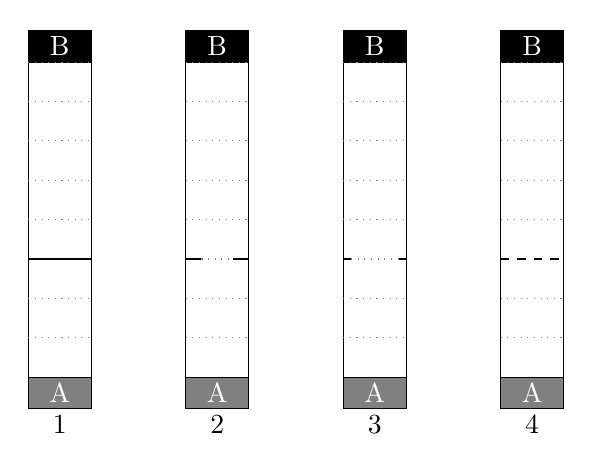
\begin{tikzpicture}
\foreach \x in {-3,-1,1,3}{

\filldraw [black] (\x, 4.0) +(-.4,0) rectangle ++(.4,0.4);
\filldraw [gray]  (\x, -.4) +(-.4,0) rectangle ++(.4,0.4);
\draw (\x, -.2) [white] node {A};
\draw (\x, 4.2) [white] node {B};
\draw [black] (\x, 0.0) +(-.4,0) -- ++(.4,0);
\draw [black] (\x, -.4) +(-.4,0) rectangle ++(.4,4.4);

\foreach \y in {0.5,1.0,2.0,2.5,3.0,3.5,4.0}
{\draw [dotted,gray] (\x,\y) +(-.4,0) -- ++(.4,0);}
}

\draw [black] (-3.4, 1.5) -- ++(.8,0);

\draw [black]  (-1.4, 1.5) -- ++(.2,0);
\draw [black]  (-0.8, 1.5) -- ++(.2,0);
\draw [dotted,gray] (-1.2, 1.5) -- ++(.4,0);


\draw [black] (0.6, 1.5) -- ++(.1,0);
\draw [black] (1.3, 1.5) -- ++(.1,0);
\draw [dotted,gray] (0.7, 1.5) -- ++(.6,0);

\draw [dashed] (2.6, 1.5) -- ++(.8,0);

\draw (-3,-.6) [black] node {1};
\draw (-1,-.6) [black] node {2};
\draw (1 ,-.6) [black] node {3};
\draw (3 ,-.6) [black] node {4};


\end{tikzpicture}